\newsection
\subsection{Healthcare and biomedicine}
\label{sec:healthcare}
\sectionauthors{Michihiro Yasunaga, Jing Huang, Camilo Ruiz, Yuhui Zhang, Giray Ogut, Saahil Jain, William Wang, Yusuf Roohani, Hongyu Ren, Antoine Bosselut, Ehsan Adeli, Jure Leskovec, Russ Altman}

% \status{second draft}

\begin{figure}[!ht]
\centering
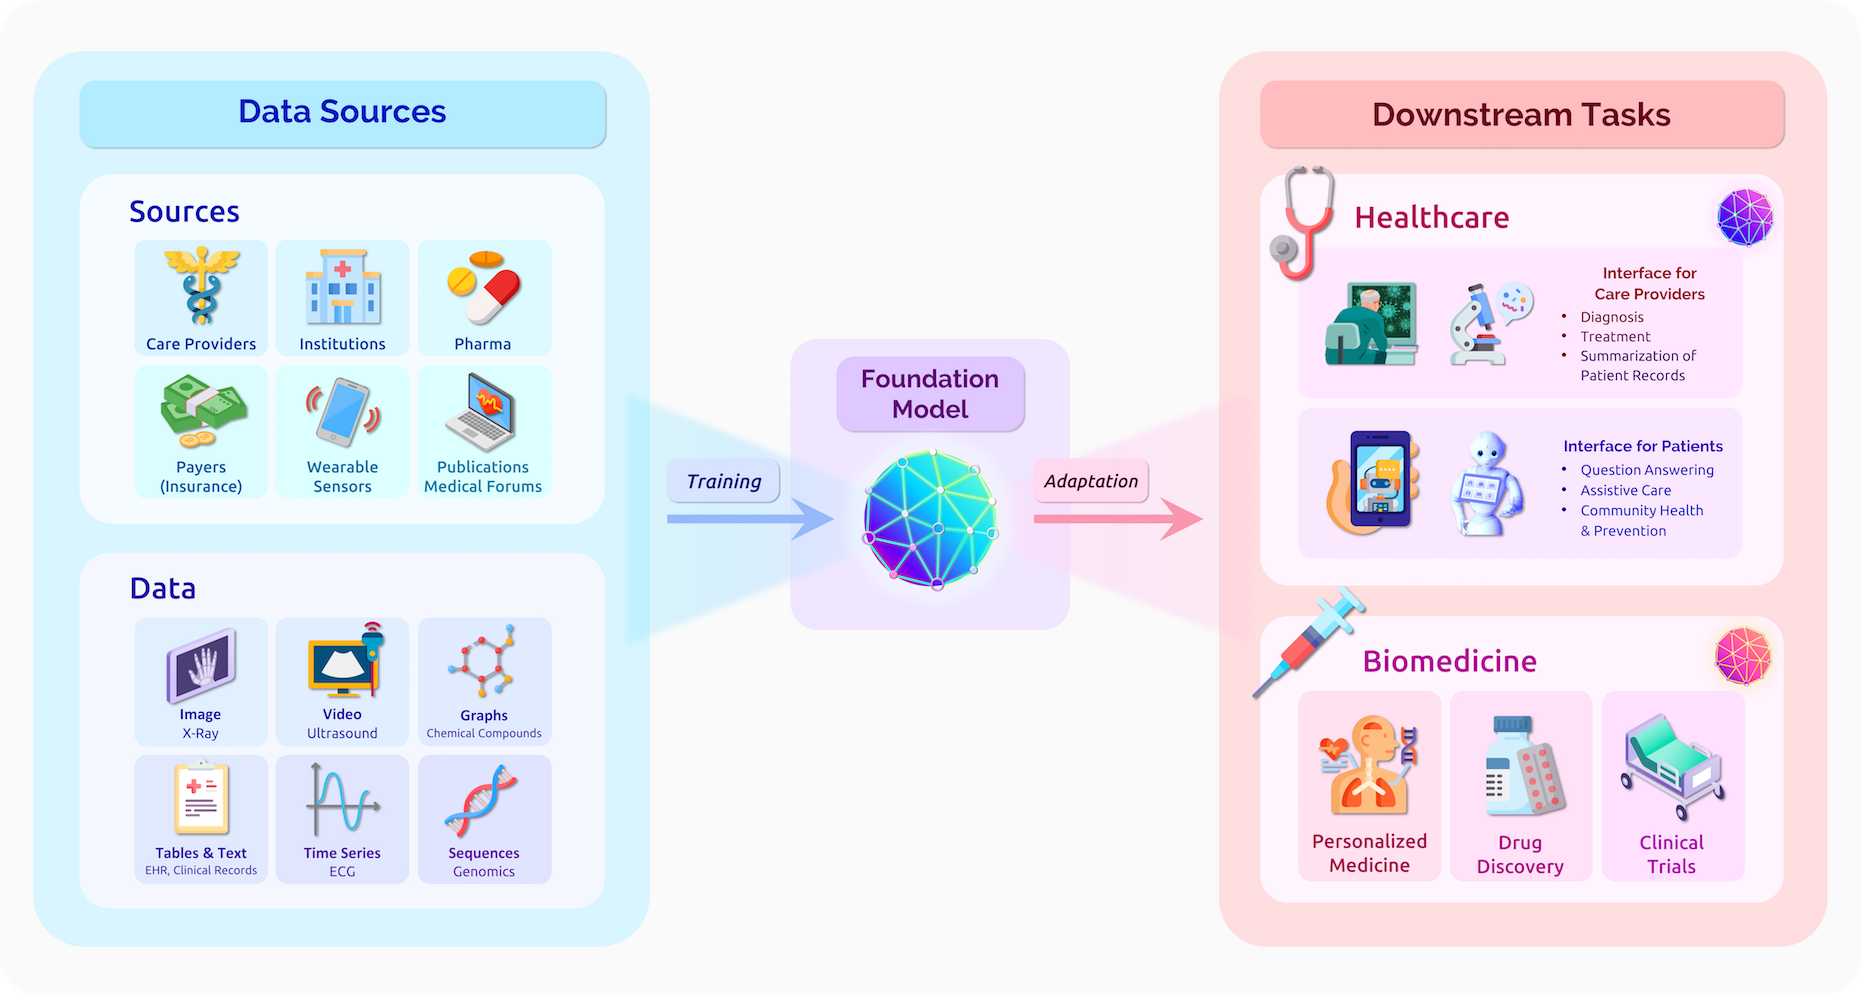
\includegraphics[width=\textwidth]{applications/healthcare_figs/Healthcare.png}
\caption{\label{fig:healthcare}
Foundation models in healthcare and biomedicine. 
We visualize an interactive framework where foundation models enable various tasks across healthcare and biomedicine when trained on multimodal data generated by various sources in the healthcare ecosystem. The first column lists several sources of data, including care providers, payers, institutions (universities, non-profits, and governments), pharma, wearables, and medical publications/forums. The second column shows several data modalities generated by the data sources. They include images (\eg chest X-rays), videos (such as ultrasounds), graphs of chemical compounds, tables for electronic health records (EHRs), text such as clinical notes, time series such as ECGs, and genetic data. The third column visualizes a foundation model trained on such data and then applied to healthcare and biomedicine downstream tasks listed in the fourth column. This process can generate new data that will further improve the foundation model, hence the bidirectional relation between the foundation models and the tasks.}
\end{figure}

Healthcare and biomedicine are an enormous application area in society, for instance, with expenditures accounting for $17$\% of gross domestic product (GDP) in the US \citep{swensen2011controlling,van_Hartskamp_2019,keehan2020national}.
Both healthcare (which focuses on the delivery of care to patients via diagnosis, treatment, and health administration) and biomedical research (which focuses on the scientific understanding of disease and the discovery of new therapies) demand significant expenses, time, and comprehensive medical knowledge \citep{yu2018artificial,korngiebel2021considering}.
We envision that foundation models can be a central storage of medical knowledge that is trained on diverse sources/modalities of data in medicine \citep{krumholz2016data,soltanian2019multimodal,suresh2020deep} (\reffig{healthcare} left), and can be queried/updated interactively by medical professionals (\eg healthcare providers and biomedical researchers access published findings and upload new publications) \citep{ionescu2020deep} and queried by the public. 
As foundation models have strong adaptation capabilities (\eg fine-tuning, prompting \citep{brown2020gpt3}), they can be efficiently adapted to various individual tasks in healthcare and biomedicine (\eg question answering app used by patients \citep{klasnja2012healthcare, zhu2019hierarchical,daniel2019towards,liu2020interpretable}, clinical trial matching system \citep{ni2015automated,harrer2019artificial,beck2020artificial} accessed by researchers and patients; \reffig{healthcare} right).
This way, foundation models can be a central interface that supports various interactions between data, tasks, and people in healthcare and biomedicine, thereby advancing the efficiency and accuracy of healthcare/biomedical applications \citep{elbattah2021role}. 
We elaborate these opportunities in \refsec{healthcare-tasks} and \refsec{biomed-tasks}.

At the same time, healthcare/biomedical applications pose unique challenges that motivate further research in foundation models, such as integrating multimodal data in healthcare/biomedicine \citep{miura2020improving,fenglincompetence2021} and observing ethical and legal regulations in medicine (privacy, safety and explainability) \citep{guan2019artificial,xu2019translating}. We elaborate these challenges in \refsec{healthcare-biomed-challenge}.


\subsubsection{Opportunities in healthcare}
\label{sec:healthcare-tasks}

Foundation models may improve the delivery of care to patients through healthcare providers and hospitals. Currently, healthcare cost increases every year \citep{keehan2020national}, and studies estimate that 30\% of healthcare spending may be wasteful due to administrative inefficiency and preventable medical errors \citep{kocher2021reducing}. Moreover, as the demand for healthcare increases, the society faces a serious shortage in healthcare providers \citep{kirch2017addressing}.
This inefficiency and shortage in healthcare necessitate developing fast and accurate interfaces for healthcare providers and patients, such as automated aid systems for diagnosis/treatment, summarization of patient records, and answering of patient questions \citep{davenport2019potential,nie2018deeptag,wang2021domain}.
In particular, in an urgent pandemic crisis such as COVID-19, fast diagnosis/screening (\eg automatic analysis of chest X-ray images) as well as automated question answering for patients (\eg symptom checking and care) and the public (\eg disease prevention) are vital to reduce the spread of diseases and allocate healthcare resources for critical patients, saving more lives \citep{lalmuanawma2020applications}.
As foundation models have a strong capability to serve as an integrated knowledge reservoir, they can be queried and adapted to various individual tasks in healthcare. Below are examples of important tasks in healthcare that would benefit from foundation models.

\paragraph{Interface for healthcare providers.} 
Foundation models can improve the efficiency and accuracy of care by providers.
Healthcare providers spend unnecessary time editing electronic heath records (EHRs) \citep{kocher2021reducing}, and preventable medical errors (\eg hospital readmissions, surgical errors) cause wastes in healthcare \citep{shrank2019waste,shah2020surgical}.
Foundation models can be adapted as an efficient and accurate interface into EHRs (clinical notes, lab value histories and imaging files) \citep{li2020behrt,steinberg2021language,percha2021modern}, helping healthcare providers create summaries of patient visitation \citep{krishna2020generating}, retrieving relevant cases and literature, and suggesting lab tests, diagnosis, treatments and discharges \citep{zhang2019vettag,rasmy2021med}. Foundation models can also be adapted to help a surgical robot monitor and achieve accurate surgeries \citep{diana2015robotic,agrigoroaie2016developing,yu2019reinforcement}. See \refsec{robotics} for more discussions on foundation models for robotics. 

\paragraph{Interface for patients.}
Foundation models can be adapted to serve as an interface to patients, providing relevant information about clinical appointments \citep{bates2019health}, answering patient questions related to preventive care \citep{demner2020consumer}, along with relevant medical explanatory information (\eg text and graphics that explain conditions) \citep{chaix2019chatbots}, and helping assistive-care robots for patients \citep{jeong2015designing,abdi2018scoping}. See \refsec{interaction} for more discussion on foundation models for user interaction. Foundation models can also serve as an interface with the general public to answer questions related to public health and pandemic prevention (such as the COVID-19 case) \citep{bharti2020medbot,herriman2020asked}. At the same time, we note that the interface must guarantee factual accuracy to ensure public trust in medical advice \citep{kreps2020model} (see \refsec{healthcare-biomed-challenge}). 



\subsubsection{Opportunities in biomedicine}
\label{sec:biomed-tasks}

Foundation models may facilitate biomedical research such as discovery of drugs and understanding of diseases, which ultimately translates to improved healthcare solutions \citep{hanney2015long}. Currently, biomedical discovery requires significant human resources, experimental time and financial costs. For instance, drug development involves a complex process,
from basic drug research of protein target identification and potent molecule discovery to clinical development (\eg clinical trials) to the final drug approval, which typically takes over 10 years and costs more than one billion dollars \citep{wouters2020estimated}.
Facilitating and accelerating biomedical discovery using existing data and published findings is an imperative problem in biomedicine \citep{yu2018artificial}. In particular, a novel disease outbreak such as COVID-19 costs millions of lives and trillions of dollars  \citep{lalmuanawma2020applications,mckibbin2020economic}; if we can speed up drug development for new diseases, that would be very helpful.
Foundation models can be particularly helpful for biomedical discovery in two aspects. First, foundation models have a strong generative capability (\eg coherent text generation in GPT-3), which can help generative tasks in biomedical research such as generating experimental protocols (clinical trials) and designing molecules that work (drug discovery) given existing data \citep{kadurin2017drugan,harrer2019artificial}. 
Second, foundation models have a potential to integrate diverse data modalities in medicine, which enables investigating biomedical concepts (\eg disease) from multiple scales (using molecule-, patient- and population-level data) and multiple knowledge sources (using imaging, textual and chemical descriptions). This facilitates biomedical discoveries that are difficult to obtain if using single-modality data \citep{lanckriet2004statistical,aerts2006gene,kong2011integrative,ribeiro2012classification,wang2014drug,wang2015kernel,ruiz2020identification,wu2021babel}.
Foundation models also enable transfer knowledge across modalities. \citet{DBLP:journals/corr/abs-2103-05247} showed how a transformer model trained on natural language (a data-rich modality) could be adapted for other sequence-based tasks such as protein fold prediction, which is a long-studied predictive task in biomedicine \citep{jumper2020high}.
Below are examples of important tasks in biomedicine that will benefit from foundation models.


\paragraph{Drug discovery.}
To discover a drug or a therapeutic that treats a disease, researchers must first identify a target (\eg proteins, genes, RNA causally implicated in the disease) and must then search for molecules (\eg chemical compounds, antibodies) that bind to the target and treat the disease. Typically, identifying the appropriate target and generating a corresponding molecule requires years of expensive wet lab experiments \citep{hughes2011principles, schenone2013target, schneider2018automating}. Foundation models' generativity can improve the search space and efficiency (see \refsec{reasoning}), which not only reduces the amount of experiments but also helps to discover new and better drugs \citep{jin2018junction, you2018graph,walters2020applications, stokes2020deep}. Moreover, the simultaneous solution of related drug discovery problems (\ie target identification, efficacy prediction, side effect prediction, and others) by a single foundation model may improve the solutions to each of them \citep{ramsundar2015massively, camacho2018next, duran2020extending, huang2021therapeutics}. As an example, one area where foundation models have shown significant potential for impacting therapeutic design is the modeling of proteins using language models. Successful applications range from predicting viral mutations that can escape a vaccine-induced immune response to predicting protein docking potential for better design of therapeutic antibodies \citep{bepler2021learning, hie2021learning, tsaban2021harnessing, wu2021protein, rives2021}.


\paragraph{Personalized medicine.}
Personalized medicine aims to select the optimal treatment for individual patients based on their health history, genetics, imaging, and other personal measurements \citep{collins2015new, ashley2016towards}.
For instance, given a set of drugs and a patient genome, foundation models may help predict which drug is likeliest to treat the patient with minimal side effects \citep{whirl2012pharmacogenomics, tatonetti2012data, gerstung2017precision, grinfeld2018classification, adam2020machine}. Foundation models are uniquely powerful in their ability to integrate multimodal patient data ranging from the EHR \citep{rajkomar2018scalable} to medical imaging \citep{bera2019artificial,ouyang2020video} to drug and molecular measurements \citep{gottlieb2011predict, ruiz2020identification} to make an optimal prediction.

\paragraph{Clinical trials.}
Clinical trials study efficacy and safety of treatment or drug candidates.
Conventional clinical trials are inefficient and costly: $80$\% of trials fail due to inability to show efficacy/safety or problems with patient matching \citep{ali2020virtual,liu2021evaluating}.
Foundation models can help in the following: predicting potential failures and design promising clinical trial protocols (\eg patient eligibility criteria) based on existing studies; and automating matching of eligible patients based on patient individual profiles, which are multimodal data including EHRs, gene sequence, etc. \citep{harrer2019artificial}.



\subsubsection{Challenges and future research in foundation models}
\label{sec:healthcare-biomed-challenge}

While there are potential opportunities for foundation models to help, healthcare/biomedical applications also pose unique challenges that motivate further research in foundation models. 

\paragraph{Multimodality.}
Medical data are highly multimodal, with various data types (text, image, video, database, molecule), scales (molecule, gene, cell, tissue, patient, population) \citep{kong2011integrative,ruiz2020identification}, and styles (professional and lay language) \citep{lavertu2019redmed,li2019neural}. Current self-supervised models are developed for each modality (\eg text~\citep{lee2020biobert}, image~\citep{chaitanya2020contrastive}, gene~\citep{ji2021dnabert}, protein~\citep{jumper2020high}), and do not jointly learn from diverse modalities.
To learn the inter-modality and cross-modality information  from these diverse multimodal medical data, we need to investigate both feature-level and semantic-level fusion strategies in the training of foundation models.
If done effectively, this has a potential to unify biomedical knowledge and facilitate discoveries as discussed in \refsec{biomed-tasks}.

\paragraph{Explainability.}
Explainability\dash{}providing evidence and logical steps for decision making\dash{}is crucial in healthcare and biomedicine \citep{holzinger2019causability}, and is made obligatory under the General Data Protection Regulation (GDPR). 
For instance, in diagnosis and clinical trials, patient symptoms and temporal relevance must be explained as evidence. This helps the resolution of potential disagreement between the system and human experts. Explainability is also needed for informed consent in healthcare \citep{amann2020explainability}.
However, current foundation models' training objectives do not include explainability, requiring future research in this direction \citep{linardatos2021explainable}. Incorporation of knowledge graphs may be a step to further improve model explainability \citep{roberts2020much, xu2020building, jin2021biomedical}.
Readers are refered to \refsec{interpretability} for more discussion on explainability.

\paragraph{Legal and ethical regulations.}
Healthcare applications must observe legal and ethical regulations with guarantees, such as patient safety, privacy and fairness. 
For instance, regarding safety, predictions made by foundation models must be factually accurate with established medical knowledge, and must quantify uncertainty or choose to defer to an expert when uncertain \citep{challen2019artificial,mozannar2020consistent}. For privacy, the use of patient health records must observe the privacy laws, such as HIPAA \citep{act1996health} in the case of the US. Federated learning is one potential solution to keeping the raw, sensitive data private in the training of foundation models \citep{chamikara2021privacy}.
For fairness, researchers will need to be mindful of common pitfalls or otherwise risk exacerbating existing social inequalities \cite{ chen2019can, wiens2019no, chen2020treating}. They must ensure that the training and evaluation data for foundation models is sufficiently representative of different sexes, races, ethnicities and socioeconomic backgrounds; an area where medical datasets and clinical trials have had a long history of bias \citep{martinez2020ethical,kaushal2020geographic}. Research is also needed to debias and regularize models to ensure fairness when representative data is scarce \cite{zhao2020training}. Foundation model developers also need to consult with ethics and law researchers, and observe regulations in the specific circumstances (\eg country, region) where they are deployed. 
We also refer readers to \refsec{security}, \refsec{robustness}, \refsec{fairness}, \refsec{legality} for details on privacy, robustness, fairness and legality. 


\paragraph{Extrapolation.}
The process of biomedical discovery involves extrapolation. For instance, foundation models must be able to quickly adapt to new experimental technologies (\eg new assays, new imaging techniques such as high resolution microscopy) or new settings (\eg new target diseases such as COVID-19) \citep{jaroch2018cell,benam2019exploring}. The ability to leverage existing datasets and extrapolate to new settings is a key machine learning challenge in biomedicine \cite{snell2017prototypical, ma2021few}. 
While GPT-3 exhibits some extrapolation behaviors (\eg generating new text not seen before), its mechanism is unclear and still in its infancy. Further research is needed for improving the extrapolation capability of foundation models, especially when considering the diverse range of data modalities and tasks that is inherent to healthcare and biomedicine but is not commonly studied in current GPT-3 and related models. Also see \refsec{robustness}. 



\iffalse %%% add citations here



\fi